\documentclass{article}%
\usepackage[T1]{fontenc}%
\usepackage[utf8]{inputenc}%
\usepackage{lmodern}%
\usepackage{textcomp}%
\usepackage{lastpage}%
\usepackage{tikz}%
%
\usepackage{tikz}%
\usetikzlibrary{shapes.multipart}%
\usepackage[a4paper, left=1in, top=1in]{geometry}%
\definecolor{mystackcolor}{HTML}{b1fa98}%
%
\begin{document}%
\normalsize%

        \section*{Implementing a Queue Using Two Stacks}
        A queue follows the First In First Out (FIFO) principle, while a stack follows the Last In First Out (LIFO) principle. We aim to mimic the behavior of a queue using two stacks.
        \subsection*{Solution Approach}
        For enqueue operation, simply push the element to stack1.
        For dequeue operation, if stack2 is empty, transfer all elements from stack1 to stack2. Then pop from stack2.
        %
\section{Enqueue(10)}%
\label{sec:Enqueue(10)}%
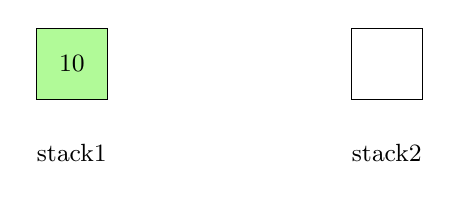
\begin{tikzpicture}%
\node[draw, fill=mystackcolor, rectangle, minimum width=0.9cm, minimum height=0.9cm] at (0, 0.0) {\fontsize{9.0pt}{9.0pt}\selectfont 10};%
\node[below] at (0, -0.9) {\fontsize{9.0pt}{9.0pt}\selectfont stack1};%
\node[draw, fill=white, rectangle, minimum width=0.9cm, minimum height=0.9cm] at (4, 0.0) {\fontsize{9.0pt}{9.0pt}\selectfont };%
\node[below] at (4, -0.9) {\fontsize{9.0pt}{9.0pt}\selectfont stack2};%
\end{tikzpicture}

%
\vspace{1cm}%
\section{Enqueue(11)}%
\label{sec:Enqueue(11)}%
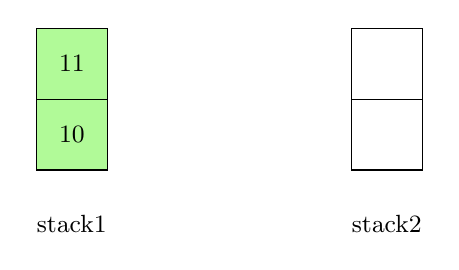
\begin{tikzpicture}%
\node[draw, fill=mystackcolor, rectangle, minimum width=0.9cm, minimum height=0.9cm] at (0, 0.0) {\fontsize{9.0pt}{9.0pt}\selectfont 11};%
\node[draw, fill=mystackcolor, rectangle, minimum width=0.9cm, minimum height=0.9cm] at (0, -0.9) {\fontsize{9.0pt}{9.0pt}\selectfont 10};%
\node[below] at (0, -1.8) {\fontsize{9.0pt}{9.0pt}\selectfont stack1};%
\node[draw, fill=white, rectangle, minimum width=0.9cm, minimum height=0.9cm] at (4, 0.0) {\fontsize{9.0pt}{9.0pt}\selectfont };%
\node[draw, fill=white, rectangle, minimum width=0.9cm, minimum height=0.9cm] at (4, -0.9) {\fontsize{9.0pt}{9.0pt}\selectfont };%
\node[below] at (4, -1.8) {\fontsize{9.0pt}{9.0pt}\selectfont stack2};%
\end{tikzpicture}

%
\vspace{1cm}%
\section{Enqueue(12)}%
\label{sec:Enqueue(12)}%
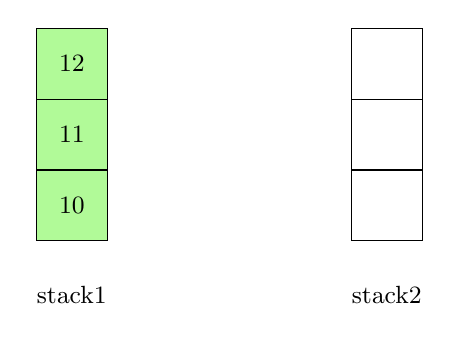
\begin{tikzpicture}%
\node[draw, fill=mystackcolor, rectangle, minimum width=0.9cm, minimum height=0.9cm] at (0, 0.0) {\fontsize{9.0pt}{9.0pt}\selectfont 12};%
\node[draw, fill=mystackcolor, rectangle, minimum width=0.9cm, minimum height=0.9cm] at (0, -0.9) {\fontsize{9.0pt}{9.0pt}\selectfont 11};%
\node[draw, fill=mystackcolor, rectangle, minimum width=0.9cm, minimum height=0.9cm] at (0, -1.8) {\fontsize{9.0pt}{9.0pt}\selectfont 10};%
\node[below] at (0, -2.7) {\fontsize{9.0pt}{9.0pt}\selectfont stack1};%
\node[draw, fill=white, rectangle, minimum width=0.9cm, minimum height=0.9cm] at (4, 0.0) {\fontsize{9.0pt}{9.0pt}\selectfont };%
\node[draw, fill=white, rectangle, minimum width=0.9cm, minimum height=0.9cm] at (4, -0.9) {\fontsize{9.0pt}{9.0pt}\selectfont };%
\node[draw, fill=white, rectangle, minimum width=0.9cm, minimum height=0.9cm] at (4, -1.8) {\fontsize{9.0pt}{9.0pt}\selectfont };%
\node[below] at (4, -2.7) {\fontsize{9.0pt}{9.0pt}\selectfont stack2};%
\end{tikzpicture}

%
\vspace{1cm}%
\section{Enqueue(13)}%
\label{sec:Enqueue(13)}%
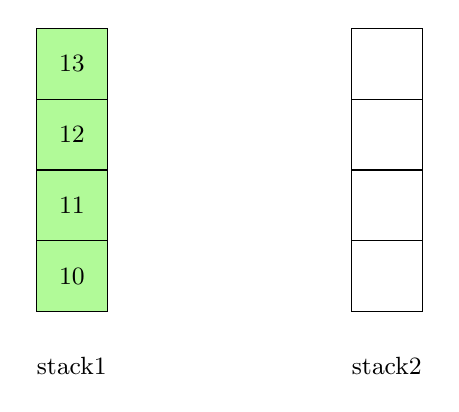
\begin{tikzpicture}%
\node[draw, fill=mystackcolor, rectangle, minimum width=0.9cm, minimum height=0.9cm] at (0, 0.0) {\fontsize{9.0pt}{9.0pt}\selectfont 13};%
\node[draw, fill=mystackcolor, rectangle, minimum width=0.9cm, minimum height=0.9cm] at (0, -0.9) {\fontsize{9.0pt}{9.0pt}\selectfont 12};%
\node[draw, fill=mystackcolor, rectangle, minimum width=0.9cm, minimum height=0.9cm] at (0, -1.8) {\fontsize{9.0pt}{9.0pt}\selectfont 11};%
\node[draw, fill=mystackcolor, rectangle, minimum width=0.9cm, minimum height=0.9cm] at (0, -2.7) {\fontsize{9.0pt}{9.0pt}\selectfont 10};%
\node[below] at (0, -3.6) {\fontsize{9.0pt}{9.0pt}\selectfont stack1};%
\node[draw, fill=white, rectangle, minimum width=0.9cm, minimum height=0.9cm] at (4, 0.0) {\fontsize{9.0pt}{9.0pt}\selectfont };%
\node[draw, fill=white, rectangle, minimum width=0.9cm, minimum height=0.9cm] at (4, -0.9) {\fontsize{9.0pt}{9.0pt}\selectfont };%
\node[draw, fill=white, rectangle, minimum width=0.9cm, minimum height=0.9cm] at (4, -1.8) {\fontsize{9.0pt}{9.0pt}\selectfont };%
\node[draw, fill=white, rectangle, minimum width=0.9cm, minimum height=0.9cm] at (4, -2.7) {\fontsize{9.0pt}{9.0pt}\selectfont };%
\node[below] at (4, -3.6) {\fontsize{9.0pt}{9.0pt}\selectfont stack2};%
\end{tikzpicture}

%
\vspace{1cm}%
\section{Enqueue(14)}%
\label{sec:Enqueue(14)}%
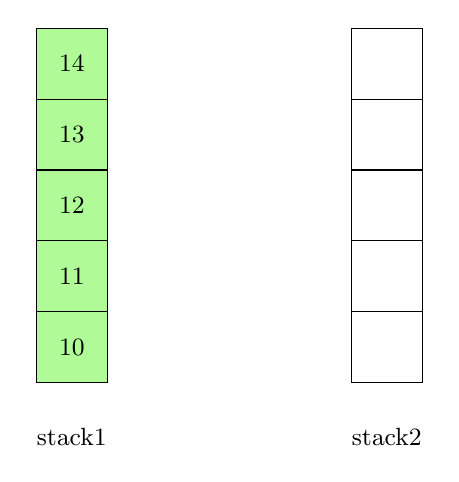
\begin{tikzpicture}%
\node[draw, fill=mystackcolor, rectangle, minimum width=0.9cm, minimum height=0.9cm] at (0, 0.0) {\fontsize{9.0pt}{9.0pt}\selectfont 14};%
\node[draw, fill=mystackcolor, rectangle, minimum width=0.9cm, minimum height=0.9cm] at (0, -0.9) {\fontsize{9.0pt}{9.0pt}\selectfont 13};%
\node[draw, fill=mystackcolor, rectangle, minimum width=0.9cm, minimum height=0.9cm] at (0, -1.8) {\fontsize{9.0pt}{9.0pt}\selectfont 12};%
\node[draw, fill=mystackcolor, rectangle, minimum width=0.9cm, minimum height=0.9cm] at (0, -2.7) {\fontsize{9.0pt}{9.0pt}\selectfont 11};%
\node[draw, fill=mystackcolor, rectangle, minimum width=0.9cm, minimum height=0.9cm] at (0, -3.6) {\fontsize{9.0pt}{9.0pt}\selectfont 10};%
\node[below] at (0, -4.5) {\fontsize{9.0pt}{9.0pt}\selectfont stack1};%
\node[draw, fill=white, rectangle, minimum width=0.9cm, minimum height=0.9cm] at (4, 0.0) {\fontsize{9.0pt}{9.0pt}\selectfont };%
\node[draw, fill=white, rectangle, minimum width=0.9cm, minimum height=0.9cm] at (4, -0.9) {\fontsize{9.0pt}{9.0pt}\selectfont };%
\node[draw, fill=white, rectangle, minimum width=0.9cm, minimum height=0.9cm] at (4, -1.8) {\fontsize{9.0pt}{9.0pt}\selectfont };%
\node[draw, fill=white, rectangle, minimum width=0.9cm, minimum height=0.9cm] at (4, -2.7) {\fontsize{9.0pt}{9.0pt}\selectfont };%
\node[draw, fill=white, rectangle, minimum width=0.9cm, minimum height=0.9cm] at (4, -3.6) {\fontsize{9.0pt}{9.0pt}\selectfont };%
\node[below] at (4, -4.5) {\fontsize{9.0pt}{9.0pt}\selectfont stack2};%
\end{tikzpicture}

%
\vspace{1cm}%
\section{Enqueue(15)}%
\label{sec:Enqueue(15)}%
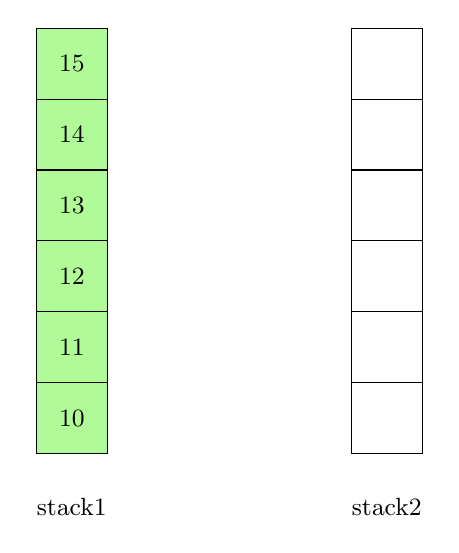
\begin{tikzpicture}%
\node[draw, fill=mystackcolor, rectangle, minimum width=0.9cm, minimum height=0.9cm] at (0, 0.0) {\fontsize{9.0pt}{9.0pt}\selectfont 15};%
\node[draw, fill=mystackcolor, rectangle, minimum width=0.9cm, minimum height=0.9cm] at (0, -0.9) {\fontsize{9.0pt}{9.0pt}\selectfont 14};%
\node[draw, fill=mystackcolor, rectangle, minimum width=0.9cm, minimum height=0.9cm] at (0, -1.8) {\fontsize{9.0pt}{9.0pt}\selectfont 13};%
\node[draw, fill=mystackcolor, rectangle, minimum width=0.9cm, minimum height=0.9cm] at (0, -2.7) {\fontsize{9.0pt}{9.0pt}\selectfont 12};%
\node[draw, fill=mystackcolor, rectangle, minimum width=0.9cm, minimum height=0.9cm] at (0, -3.6) {\fontsize{9.0pt}{9.0pt}\selectfont 11};%
\node[draw, fill=mystackcolor, rectangle, minimum width=0.9cm, minimum height=0.9cm] at (0, -4.5) {\fontsize{9.0pt}{9.0pt}\selectfont 10};%
\node[below] at (0, -5.4) {\fontsize{9.0pt}{9.0pt}\selectfont stack1};%
\node[draw, fill=white, rectangle, minimum width=0.9cm, minimum height=0.9cm] at (4, 0.0) {\fontsize{9.0pt}{9.0pt}\selectfont };%
\node[draw, fill=white, rectangle, minimum width=0.9cm, minimum height=0.9cm] at (4, -0.9) {\fontsize{9.0pt}{9.0pt}\selectfont };%
\node[draw, fill=white, rectangle, minimum width=0.9cm, minimum height=0.9cm] at (4, -1.8) {\fontsize{9.0pt}{9.0pt}\selectfont };%
\node[draw, fill=white, rectangle, minimum width=0.9cm, minimum height=0.9cm] at (4, -2.7) {\fontsize{9.0pt}{9.0pt}\selectfont };%
\node[draw, fill=white, rectangle, minimum width=0.9cm, minimum height=0.9cm] at (4, -3.6) {\fontsize{9.0pt}{9.0pt}\selectfont };%
\node[draw, fill=white, rectangle, minimum width=0.9cm, minimum height=0.9cm] at (4, -4.5) {\fontsize{9.0pt}{9.0pt}\selectfont };%
\node[below] at (4, -5.4) {\fontsize{9.0pt}{9.0pt}\selectfont stack2};%
\end{tikzpicture}

%
\vspace{1cm}%
\section{Transferred stack1 to stack2}%
\label{sec:Transferredstack1tostack2}%
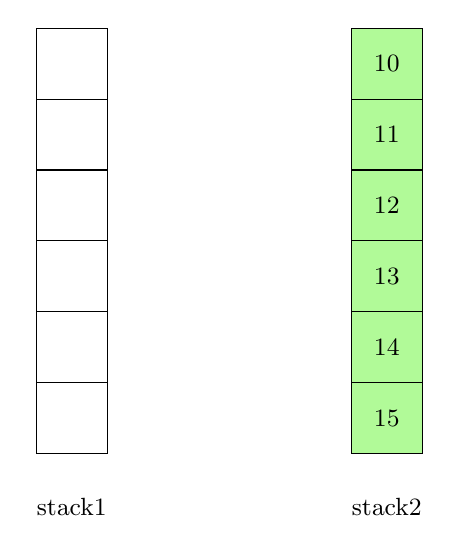
\begin{tikzpicture}%
\node[draw, fill=white, rectangle, minimum width=0.9cm, minimum height=0.9cm] at (0, 0.0) {\fontsize{9.0pt}{9.0pt}\selectfont };%
\node[draw, fill=white, rectangle, minimum width=0.9cm, minimum height=0.9cm] at (0, -0.9) {\fontsize{9.0pt}{9.0pt}\selectfont };%
\node[draw, fill=white, rectangle, minimum width=0.9cm, minimum height=0.9cm] at (0, -1.8) {\fontsize{9.0pt}{9.0pt}\selectfont };%
\node[draw, fill=white, rectangle, minimum width=0.9cm, minimum height=0.9cm] at (0, -2.7) {\fontsize{9.0pt}{9.0pt}\selectfont };%
\node[draw, fill=white, rectangle, minimum width=0.9cm, minimum height=0.9cm] at (0, -3.6) {\fontsize{9.0pt}{9.0pt}\selectfont };%
\node[draw, fill=white, rectangle, minimum width=0.9cm, minimum height=0.9cm] at (0, -4.5) {\fontsize{9.0pt}{9.0pt}\selectfont };%
\node[below] at (0, -5.4) {\fontsize{9.0pt}{9.0pt}\selectfont stack1};%
\node[draw, fill=mystackcolor, rectangle, minimum width=0.9cm, minimum height=0.9cm] at (4, 0.0) {\fontsize{9.0pt}{9.0pt}\selectfont 10};%
\node[draw, fill=mystackcolor, rectangle, minimum width=0.9cm, minimum height=0.9cm] at (4, -0.9) {\fontsize{9.0pt}{9.0pt}\selectfont 11};%
\node[draw, fill=mystackcolor, rectangle, minimum width=0.9cm, minimum height=0.9cm] at (4, -1.8) {\fontsize{9.0pt}{9.0pt}\selectfont 12};%
\node[draw, fill=mystackcolor, rectangle, minimum width=0.9cm, minimum height=0.9cm] at (4, -2.7) {\fontsize{9.0pt}{9.0pt}\selectfont 13};%
\node[draw, fill=mystackcolor, rectangle, minimum width=0.9cm, minimum height=0.9cm] at (4, -3.6) {\fontsize{9.0pt}{9.0pt}\selectfont 14};%
\node[draw, fill=mystackcolor, rectangle, minimum width=0.9cm, minimum height=0.9cm] at (4, -4.5) {\fontsize{9.0pt}{9.0pt}\selectfont 15};%
\node[below] at (4, -5.4) {\fontsize{9.0pt}{9.0pt}\selectfont stack2};%
\end{tikzpicture}

%
\vspace{1cm}%
\section{Dequeue(): 10}%
\label{sec:Dequeue()10}%
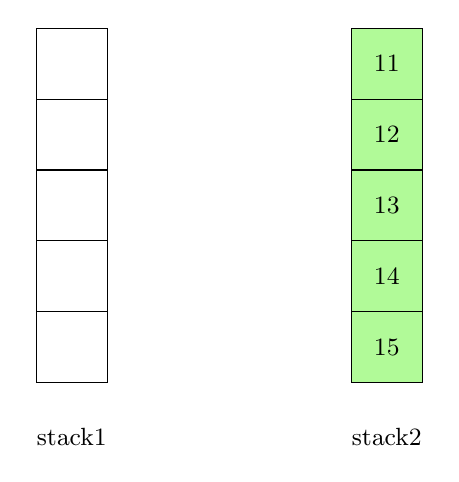
\begin{tikzpicture}%
\node[draw, fill=white, rectangle, minimum width=0.9cm, minimum height=0.9cm] at (0, 0.0) {\fontsize{9.0pt}{9.0pt}\selectfont };%
\node[draw, fill=white, rectangle, minimum width=0.9cm, minimum height=0.9cm] at (0, -0.9) {\fontsize{9.0pt}{9.0pt}\selectfont };%
\node[draw, fill=white, rectangle, minimum width=0.9cm, minimum height=0.9cm] at (0, -1.8) {\fontsize{9.0pt}{9.0pt}\selectfont };%
\node[draw, fill=white, rectangle, minimum width=0.9cm, minimum height=0.9cm] at (0, -2.7) {\fontsize{9.0pt}{9.0pt}\selectfont };%
\node[draw, fill=white, rectangle, minimum width=0.9cm, minimum height=0.9cm] at (0, -3.6) {\fontsize{9.0pt}{9.0pt}\selectfont };%
\node[below] at (0, -4.5) {\fontsize{9.0pt}{9.0pt}\selectfont stack1};%
\node[draw, fill=mystackcolor, rectangle, minimum width=0.9cm, minimum height=0.9cm] at (4, 0.0) {\fontsize{9.0pt}{9.0pt}\selectfont 11};%
\node[draw, fill=mystackcolor, rectangle, minimum width=0.9cm, minimum height=0.9cm] at (4, -0.9) {\fontsize{9.0pt}{9.0pt}\selectfont 12};%
\node[draw, fill=mystackcolor, rectangle, minimum width=0.9cm, minimum height=0.9cm] at (4, -1.8) {\fontsize{9.0pt}{9.0pt}\selectfont 13};%
\node[draw, fill=mystackcolor, rectangle, minimum width=0.9cm, minimum height=0.9cm] at (4, -2.7) {\fontsize{9.0pt}{9.0pt}\selectfont 14};%
\node[draw, fill=mystackcolor, rectangle, minimum width=0.9cm, minimum height=0.9cm] at (4, -3.6) {\fontsize{9.0pt}{9.0pt}\selectfont 15};%
\node[below] at (4, -4.5) {\fontsize{9.0pt}{9.0pt}\selectfont stack2};%
\end{tikzpicture}

%
\vspace{1cm}%
\section{Dequeue(): 11}%
\label{sec:Dequeue()11}%
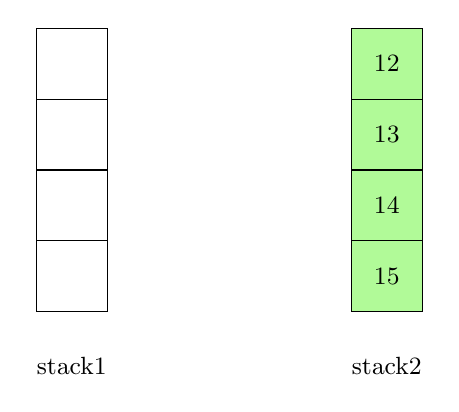
\begin{tikzpicture}%
\node[draw, fill=white, rectangle, minimum width=0.9cm, minimum height=0.9cm] at (0, 0.0) {\fontsize{9.0pt}{9.0pt}\selectfont };%
\node[draw, fill=white, rectangle, minimum width=0.9cm, minimum height=0.9cm] at (0, -0.9) {\fontsize{9.0pt}{9.0pt}\selectfont };%
\node[draw, fill=white, rectangle, minimum width=0.9cm, minimum height=0.9cm] at (0, -1.8) {\fontsize{9.0pt}{9.0pt}\selectfont };%
\node[draw, fill=white, rectangle, minimum width=0.9cm, minimum height=0.9cm] at (0, -2.7) {\fontsize{9.0pt}{9.0pt}\selectfont };%
\node[below] at (0, -3.6) {\fontsize{9.0pt}{9.0pt}\selectfont stack1};%
\node[draw, fill=mystackcolor, rectangle, minimum width=0.9cm, minimum height=0.9cm] at (4, 0.0) {\fontsize{9.0pt}{9.0pt}\selectfont 12};%
\node[draw, fill=mystackcolor, rectangle, minimum width=0.9cm, minimum height=0.9cm] at (4, -0.9) {\fontsize{9.0pt}{9.0pt}\selectfont 13};%
\node[draw, fill=mystackcolor, rectangle, minimum width=0.9cm, minimum height=0.9cm] at (4, -1.8) {\fontsize{9.0pt}{9.0pt}\selectfont 14};%
\node[draw, fill=mystackcolor, rectangle, minimum width=0.9cm, minimum height=0.9cm] at (4, -2.7) {\fontsize{9.0pt}{9.0pt}\selectfont 15};%
\node[below] at (4, -3.6) {\fontsize{9.0pt}{9.0pt}\selectfont stack2};%
\end{tikzpicture}

%
\vspace{1cm}%
\section{Dequeue(): 12}%
\label{sec:Dequeue()12}%
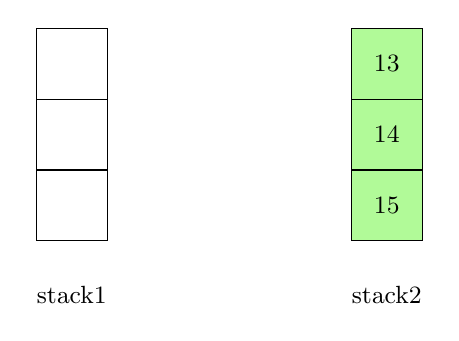
\begin{tikzpicture}%
\node[draw, fill=white, rectangle, minimum width=0.9cm, minimum height=0.9cm] at (0, 0.0) {\fontsize{9.0pt}{9.0pt}\selectfont };%
\node[draw, fill=white, rectangle, minimum width=0.9cm, minimum height=0.9cm] at (0, -0.9) {\fontsize{9.0pt}{9.0pt}\selectfont };%
\node[draw, fill=white, rectangle, minimum width=0.9cm, minimum height=0.9cm] at (0, -1.8) {\fontsize{9.0pt}{9.0pt}\selectfont };%
\node[below] at (0, -2.7) {\fontsize{9.0pt}{9.0pt}\selectfont stack1};%
\node[draw, fill=mystackcolor, rectangle, minimum width=0.9cm, minimum height=0.9cm] at (4, 0.0) {\fontsize{9.0pt}{9.0pt}\selectfont 13};%
\node[draw, fill=mystackcolor, rectangle, minimum width=0.9cm, minimum height=0.9cm] at (4, -0.9) {\fontsize{9.0pt}{9.0pt}\selectfont 14};%
\node[draw, fill=mystackcolor, rectangle, minimum width=0.9cm, minimum height=0.9cm] at (4, -1.8) {\fontsize{9.0pt}{9.0pt}\selectfont 15};%
\node[below] at (4, -2.7) {\fontsize{9.0pt}{9.0pt}\selectfont stack2};%
\end{tikzpicture}

%
\vspace{1cm}%
\section{Dequeue(): 13}%
\label{sec:Dequeue()13}%
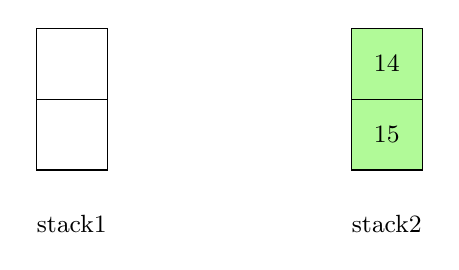
\begin{tikzpicture}%
\node[draw, fill=white, rectangle, minimum width=0.9cm, minimum height=0.9cm] at (0, 0.0) {\fontsize{9.0pt}{9.0pt}\selectfont };%
\node[draw, fill=white, rectangle, minimum width=0.9cm, minimum height=0.9cm] at (0, -0.9) {\fontsize{9.0pt}{9.0pt}\selectfont };%
\node[below] at (0, -1.8) {\fontsize{9.0pt}{9.0pt}\selectfont stack1};%
\node[draw, fill=mystackcolor, rectangle, minimum width=0.9cm, minimum height=0.9cm] at (4, 0.0) {\fontsize{9.0pt}{9.0pt}\selectfont 14};%
\node[draw, fill=mystackcolor, rectangle, minimum width=0.9cm, minimum height=0.9cm] at (4, -0.9) {\fontsize{9.0pt}{9.0pt}\selectfont 15};%
\node[below] at (4, -1.8) {\fontsize{9.0pt}{9.0pt}\selectfont stack2};%
\end{tikzpicture}

%
\vspace{1cm}%
\section{Dequeue(): 14}%
\label{sec:Dequeue()14}%
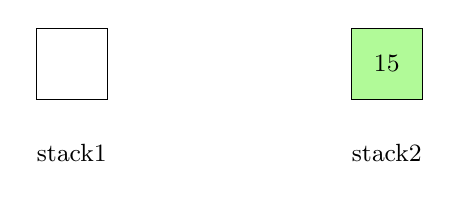
\begin{tikzpicture}%
\node[draw, fill=white, rectangle, minimum width=0.9cm, minimum height=0.9cm] at (0, 0.0) {\fontsize{9.0pt}{9.0pt}\selectfont };%
\node[below] at (0, -0.9) {\fontsize{9.0pt}{9.0pt}\selectfont stack1};%
\node[draw, fill=mystackcolor, rectangle, minimum width=0.9cm, minimum height=0.9cm] at (4, 0.0) {\fontsize{9.0pt}{9.0pt}\selectfont 15};%
\node[below] at (4, -0.9) {\fontsize{9.0pt}{9.0pt}\selectfont stack2};%
\end{tikzpicture}

%
\vspace{1cm}%
\section{Dequeue(): 15}%
\label{sec:Dequeue()15}%
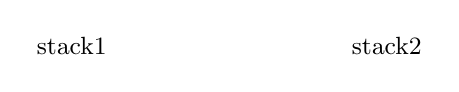
\begin{tikzpicture}%
\node[below] at (0, 0.0) {\fontsize{9.0pt}{9.0pt}\selectfont stack1};%
\node[below] at (4, 0.0) {\fontsize{9.0pt}{9.0pt}\selectfont stack2};%
\end{tikzpicture}

%
\vspace{1cm}%
\end{document}